\documentclass[12pt,a4paper]{book}

% ==================== PACKAGES ====================
\usepackage[utf8]{inputenc}
\usepackage[T1]{fontenc}
\usepackage{geometry}
\usepackage{xcolor}
\usepackage{graphicx}
\usepackage{tikz}
\usepackage{tcolorbox}
\usepackage{fancyhdr}
\usepackage{titlesec}
\usepackage{hyperref}
\usepackage{enumitem}
\usepackage{booktabs}
\usepackage{longtable}
\usepackage{array}
\usepackage{float}
\usepackage{caption}
\usepackage{pgfplots}

\usetikzlibrary{shapes,arrows,positioning,shadows,patterns,calc}
\pgfplotsset{compat=1.18}

% ==================== COLOR DEFINITIONS ====================
% NVIDIA Colors
\definecolor{nvidiagreen}{HTML}{76b900}
\definecolor{nvidiablack}{HTML}{000000}
\definecolor{nvidiawhite}{HTML}{FFFFFF}
\definecolor{nvidiadarkgray}{HTML}{1A1A1A}
\definecolor{nvidialightgray}{HTML}{666666}

% Microsoft Theme Colors
\definecolor{msblue}{HTML}{0078D4}
\definecolor{msred}{HTML}{D83B01}
\definecolor{msyellow}{HTML}{FFB900}
\definecolor{msgreen}{HTML}{107C10}

% ==================== PAGE GEOMETRY ====================
\geometry{
    a4paper,
    left=2.5cm,
    right=2.5cm,
    top=3cm,
    bottom=3cm,
    headheight=15pt
}

% ==================== HYPERREF SETUP ====================
\hypersetup{
    colorlinks=true,
    linkcolor=nvidiagreen,
    urlcolor=msblue,
    citecolor=nvidiagreen,
    filecolor=nvidiagreen,
    pdftitle={NVIDIA GPU Architecture Guide},
    pdfauthor={Yash Kavaiya},
    pdfsubject={NVIDIA GPU Technology},
    pdfkeywords={NVIDIA, GPU, AI, Machine Learning}
}

% ==================== HEADER AND FOOTER ====================
\pagestyle{fancy}
\fancyhf{}
\fancyhead[L]{\textcolor{nvidiagreen}{\leftmark}}
\fancyhead[R]{\textcolor{nvidiagreen}{\thepage}}
\fancyfoot[L]{\small\href{https://easy-ai-labs.lovable.app/}{\textcolor{msblue}{Easy AI Labs}}}
\fancyfoot[C]{\small\href{https://www.linkedin.com/in/yashkavaiya}{\textcolor{msblue}{Yash Kavaiya}}}
\fancyfoot[R]{\small\href{https://www.linkedin.com/company/genai-guru}{\textcolor{msblue}{Gen AI Guru}}}
\renewcommand{\headrulewidth}{2pt}
\renewcommand{\footrulewidth}{1pt}
\renewcommand{\headrule}{\hbox to\headwidth{\color{nvidiagreen}\leaders\hrule height \headrulewidth\hfill}}
\renewcommand{\footrule}{\hbox to\headwidth{\color{nvidiagreen}\leaders\hrule height \footrulewidth\hfill}}

% ==================== TITLE FORMATTING ====================
\titleformat{\chapter}[display]
{\normalfont\huge\bfseries\color{nvidiagreen}}
{\filleft\Huge\thechapter}
{2ex}
{\titlerule\vspace{1ex}\filleft}
[\vspace{1ex}\titlerule]

\titleformat{\section}
{\normalfont\Large\bfseries\color{nvidiagreen}}
{\thesection}{1em}{}

\titleformat{\subsection}
{\normalfont\large\bfseries\color{msblue}}
{\thesubsection}{1em}{}

% ==================== CUSTOM BOXES ====================
\newtcolorbox{nvidiabox}[1][]{
    colback=nvidiadarkgray,
    colframe=nvidiagreen,
    fonttitle=\bfseries\color{nvidiawhite},
    coltitle=nvidiawhite,
    title=#1,
    arc=3mm,
    boxrule=2pt
}

\newtcolorbox{msbox}[1][]{
    colback=msblue!10,
    colframe=msblue,
    fonttitle=\bfseries,
    title=#1,
    arc=2mm,
    boxrule=1.5pt
}

% ==================== DOCUMENT BEGIN ====================
\begin{document}

% ==================== TITLE PAGE ====================
\begin{titlepage}
    \begin{tikzpicture}[remember picture,overlay]
        \fill[nvidiablack] (current page.south west) rectangle (current page.north east);
        
        % NVIDIA Green accent bars
        \fill[nvidiagreen] (current page.north west) rectangle ([yshift=-2cm]current page.north east);
        \fill[nvidiagreen] ([yshift=2cm]current page.south west) rectangle (current page.south east);
        
        % Microsoft color accents
        \fill[msblue] ([xshift=2cm,yshift=-2.5cm]current page.north west) rectangle ([xshift=3cm,yshift=-3cm]current page.north west);
        \fill[msred] ([xshift=3.5cm,yshift=-2.5cm]current page.north west) rectangle ([xshift=4.5cm,yshift=-3cm]current page.north west);
        \fill[msyellow] ([xshift=5cm,yshift=-2.5cm]current page.north west) rectangle ([xshift=6cm,yshift=-3cm]current page.north west);
        \fill[msgreen] ([xshift=6.5cm,yshift=-2.5cm]current page.north west) rectangle ([xshift=7.5cm,yshift=-3cm]current page.north west);
        
        \node[anchor=center] at (current page.center) {
            \begin{minipage}{\textwidth}
                \centering
                {\Huge\bfseries\color{nvidiagreen} NVIDIA GPU}\\[0.5cm]
                {\Huge\bfseries\color{nvidiawhite} Architecture Guide}\\[1.5cm]
                {\Large\color{nvidialightgray} From Foundation to Future}\\[0.5cm]
                {\Large\color{nvidialightgray} Deep Learning Systems \& AI Infrastructure}\\[3cm]
                {\large\color{nvidiawhite} Authored by}\\[0.3cm]
                {\Large\bfseries\color{nvidiagreen} Yash Kavaiya}\\[0.5cm]
                {\large\color{nvidiawhite} \href{https://easy-ai-labs.lovable.app/}{Easy AI Labs} | \href{https://www.linkedin.com/company/genai-guru}{Gen AI Guru}}
            \end{minipage}
        };
    \end{tikzpicture}
\end{titlepage}

% ==================== TABLE OF CONTENTS ====================
\tableofcontents
\newpage

% ==================== CHAPTER 1: INTRODUCTION ====================
\chapter{Introduction to NVIDIA GPU Evolution}

\section{Historical Timeline}

NVIDIA's journey from a graphics card manufacturer to an AI powerhouse represents one of the most remarkable transformations in technology history. This chapter explores the key milestones that shaped NVIDIA's evolution.

\begin{nvidiabox}[NVIDIA Evolution Timeline]
    \textcolor{nvidiawhite}{
    \textbf{Foundation Era} → \textbf{CUDA Revolution} → \textbf{Ray Tracing} → \textbf{Data Center} → \textbf{AI Dominance}
    }
\end{nvidiabox}

\subsection{Key Milestones}

\begin{table}[H]
\centering
\caption{NVIDIA Major Product Launches}
\begin{tabular}{@{}lll@{}}
\toprule
\textbf{Year} & \textbf{Product/Technology} & \textbf{Significance} \\ \midrule
\textcolor{nvidiagreen}{\textbf{1993}} & Company Founded & Graphics processing begins \\
\textcolor{nvidiagreen}{\textbf{2007}} & CUDA Platform & Parallel computing revolution \\
\textcolor{nvidiagreen}{\textbf{2018}} & RTX Technology & Real-time ray tracing \\
\textcolor{nvidiagreen}{\textbf{2020}} & A100 Data Center GPU & AI training acceleration \\
\textcolor{nvidiagreen}{\textbf{2022}} & H100 Hopper & Most popular AI GPU \\
\textcolor{nvidiagreen}{\textbf{2025}} & Blackwell Architecture & Next-gen AI infrastructure \\
\textcolor{nvidiagreen}{\textbf{Future}} & Rubin \& Vera & Upcoming platforms \\ \bottomrule
\end{tabular}
\end{table}

\section{Technology Evolution Diagram}

\begin{figure}[H]
\centering
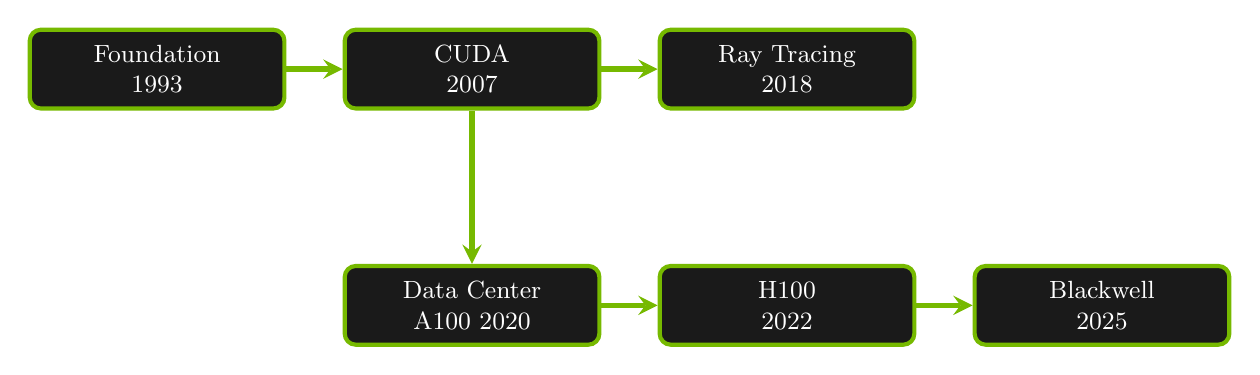
\begin{tikzpicture}[
    node distance=2cm,
    every node/.style={font=\small},
    block/.style={rectangle, draw=nvidiagreen, fill=nvidiadarkgray, text=nvidiawhite, 
                  text width=3cm, text centered, rounded corners, minimum height=1cm, line width=1.5pt},
    arrow/.style={->, >=stealth, line width=2pt, color=nvidiagreen}
]
    \node[block] (foundation) {Foundation\\1993};
    \node[block, right of=foundation, xshift=2cm] (cuda) {CUDA\\2007};
    \node[block, right of=cuda, xshift=2cm] (raytracing) {Ray Tracing\\2018};
    \node[block, below of=cuda, yshift=-1cm] (datacenter) {Data Center\\A100 2020};
    \node[block, right of=datacenter, xshift=2cm] (h100) {H100\\2022};
    \node[block, right of=h100, xshift=2cm] (blackwell) {Blackwell\\2025};
    
    \draw[arrow] (foundation) -- (cuda);
    \draw[arrow] (cuda) -- (raytracing);
    \draw[arrow] (cuda) -- (datacenter);
    \draw[arrow] (datacenter) -- (h100);
    \draw[arrow] (h100) -- (blackwell);
\end{tikzpicture}
\caption{NVIDIA Technology Evolution Path}
\end{figure}

% ==================== CHAPTER 2: DGX SYSTEMS ====================
\chapter{NVIDIA DGX Systems}

\section{Overview of DGX Platform}

NVIDIA DGX systems represent the pinnacle of deep learning infrastructure, specifically engineered for AI, ML, and neural network workloads. These systems integrate optimized hardware and software to deliver unprecedented performance.

\begin{msbox}[DGX Definition]
\textbf{DGX (Deep Learning GPU eXtension)} is NVIDIA's purpose-built platform designed specifically for AI, Machine Learning, and Neural Network workloads, combining cutting-edge GPUs with optimized system architecture.
\end{msbox}

\subsection{DGX System Form Factors}

\begin{figure}[H]
\centering

\begin{tikzpicture}
    % Large Server
    \draw[fill=nvidiadarkgray, draw=nvidiagreen, line width=2pt] (0,0) rectangle (3,2);
    \node[text=nvidiawhite, font=\bfseries] at (1.5,1) {Large Server};
    
    % Medium Server
    \draw[fill=nvidiadarkgray, draw=msblue, line width=2pt] (4,0) rectangle (6.5,2);
    \node[text=nvidiawhite, font=\bfseries] at (5.25,1) {Rack Server};
    
    % Desktop
    \draw[fill=nvidiadarkgray, draw=msred, line width=2pt] (7.5,0) rectangle (10,2);
    \node[text=nvidiawhite, font=\bfseries] at (8.75,1) {Workstation};
\end{tikzpicture}
\caption{DGX System Form Factors}
\end{figure}

\section{DGX Evolution Timeline}

\begin{table}[H]
\centering
\caption{DGX System Evolution (2016-Present)}
\begin{tabular}{@{}llll@{}}
\toprule
\textbf{System} & \textbf{Year} & \textbf{CPU} & \textbf{GPU} \\ \midrule
\textcolor{nvidiagreen}{\textbf{DGX-1}} & 2016 & Intel & Tesla P100 \\
\textcolor{nvidiagreen}{\textbf{DGX-2}} & 2018 & Intel & Tesla V100 \\
\textcolor{msblue}{\textbf{DGX A100}} & 2020 & AMD EPYC & A100 Ampere \\
\textcolor{msblue}{\textbf{DGX H100}} & 2022 & Intel Xeon & H100 Hopper \\
\textcolor{nvidiagreen}{\textbf{DGX GH200}} & 2023 & Grace ARM & H200 Hopper \\
\textcolor{nvidiagreen}{\textbf{DGX GB200}} & 2024 & Grace ARM & Blackwell \\ \bottomrule
\end{tabular}
\end{table}

\subsection{CPU-GPU Combinations}

\begin{nvidiabox}[DGX Naming Convention]
\textcolor{nvidiawhite}{
\textbf{Grace Hopper 200 (GH200):}\\
• \textbf{G} = Grace (NVIDIA ARM CPU)\\
• \textbf{H} = Hopper (NVIDIA GPU Architecture)\\
• \textbf{200} = Generation/Series Number
}
\end{nvidiabox}

% ==================== CHAPTER 3: GRACE CPU ====================
\chapter{NVIDIA Grace CPU Architecture}

\section{Grace CPU Specifications}

NVIDIA Grace represents a paradigm shift in CPU design, bringing ARM-based architecture to high-performance computing with unprecedented integration with GPU technology.

\begin{table}[H]
\centering
\caption{NVIDIA Grace CPU Technical Specifications}
\begin{tabular}{@{}ll@{}}
\toprule
\textbf{Specification} & \textbf{Details} \\ \midrule
\textcolor{nvidiagreen}{\textbf{Core Count}} & 72 ARM Neoverse cores \\
\textcolor{nvidiagreen}{\textbf{Architecture}} & ARM-based custom design \\
\textcolor{nvidiagreen}{\textbf{Memory}} & LPDDR5X support \\
\textcolor{nvidiagreen}{\textbf{Bandwidth}} & 512 GB/s memory bandwidth \\
\textcolor{nvidiagreen}{\textbf{Interconnect}} & NVLink-C2C technology \\
\textcolor{nvidiagreen}{\textbf{PCI Express}} & PCIe Gen 5.0 support \\
\textcolor{nvidiagreen}{\textbf{Power Efficiency}} & Optimized for AI workloads \\ \bottomrule
\end{tabular}
\end{table}

\section{Grace Hopper Superchip Architecture}

\begin{figure}[H]
\centering
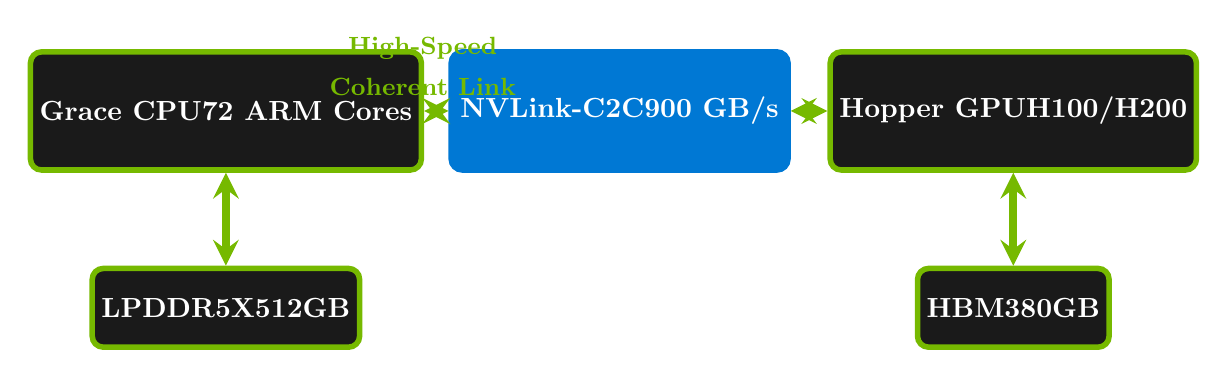
\begin{tikzpicture}[
    component/.style={rectangle, draw=nvidiagreen, fill=nvidiadarkgray, text=nvidiawhite,
                      minimum width=3.5cm, minimum height=1.5cm, line width=2pt,
                      rounded corners, font=\bfseries},
    connection/.style={<->, >=stealth, line width=3pt, color=nvidiagreen}
]
    % Grace CPU
    \node[component] (grace) at (0,0) {Grace CPU\\72 ARM Cores};
    
    % NVLink Connection
    \node[component, fill=msblue, draw=msblue] (nvlink) at (5,0) {NVLink-C2C\\900 GB/s};
    
    % Hopper GPU
    \node[component] (hopper) at (10,0) {Hopper GPU\\H100/H200};
    
    % Memory components
    \node[component, minimum width=2cm, minimum height=1cm] (gracemem) at (0,-2.5) {LPDDR5X\\512GB};
    \node[component, minimum width=2cm, minimum height=1cm] (gpumem) at (10,-2.5) {HBM3\\80GB};
    
    % Connections
    \draw[connection] (grace) -- (nvlink);
    \draw[connection] (nvlink) -- (hopper);
    \draw[connection] (grace) -- (gracemem);
    \draw[connection] (hopper) -- (gpumem);
    
    % Labels
    \node[text=nvidiagreen, font=\small\bfseries] at (2.5,0.8) {High-Speed};
    \node[text=nvidiagreen, font=\small\bfseries] at (2.5,0.3) {Coherent Link};
\end{tikzpicture}
\caption{Grace Hopper Superchip Architecture}
\end{figure}

\subsection{Key Technological Advantages}

\begin{enumerate}[label=\textcolor{nvidiagreen}{\arabic*.}, leftmargin=*]
    \item \textbf{Coherent Memory Access:} NVLink-C2C enables seamless memory sharing between CPU and GPU
    \item \textbf{High Bandwidth:} 900 GB/s bidirectional bandwidth eliminates CPU-GPU bottlenecks
    \item \textbf{Energy Efficiency:} ARM architecture provides superior performance-per-watt
    \item \textbf{Unified Architecture:} Optimized for AI/ML workloads from the ground up
\end{enumerate}

\section{Performance Comparison}

\begin{figure}[H]
\centering
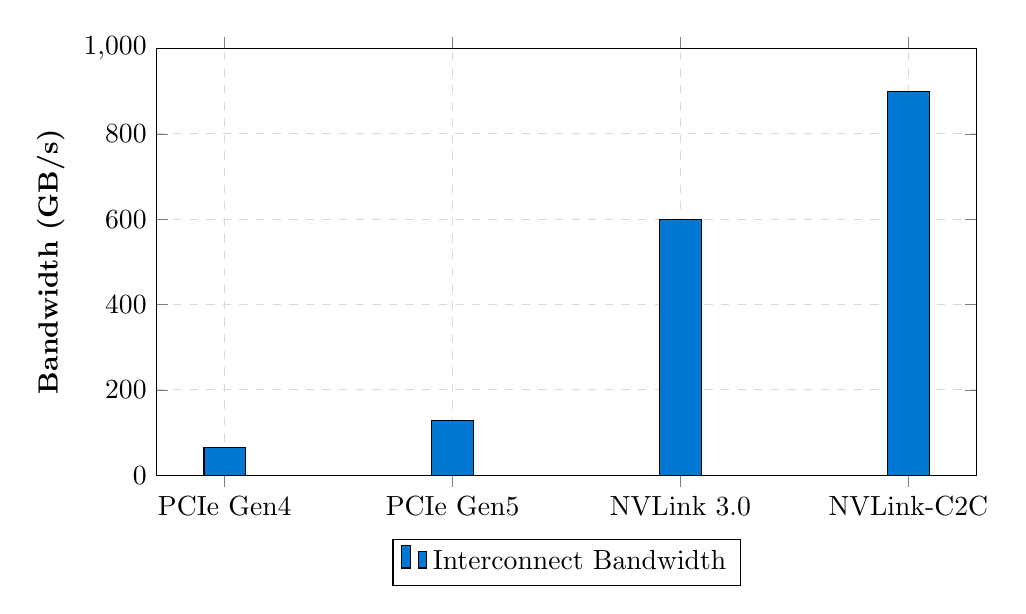
\begin{tikzpicture}
\begin{axis}[
    ybar,
    bar width=15pt,
    width=12cm,
    height=7cm,
    ylabel={Bandwidth (GB/s)},
    symbolic x coords={PCIe Gen4, PCIe Gen5, NVLink 3.0, NVLink-C2C},
    xtick=data,
    ymin=0,
    ymax=1000,
    legend style={at={(0.5,-0.15)}, anchor=north, legend columns=-1},
    ylabel style={font=\bfseries},
    xlabel style={font=\bfseries},
    grid=major,
    grid style={dashed,gray!30}
]
\addplot[fill=msblue] coordinates {(PCIe Gen4,64) (PCIe Gen5,128) (NVLink 3.0,600) (NVLink-C2C,900)};
\legend{Interconnect Bandwidth}
\end{axis}
\end{tikzpicture}
\caption{Interconnect Technology Comparison}
\end{figure}

% ==================== CHAPTER 4: COMPUTE PORTFOLIO ====================
\chapter{NVIDIA Compute Portfolio}

\section{GPU Lineup Overview}

NVIDIA offers a comprehensive portfolio of GPU solutions optimized for different workloads, from training large language models to inference and analytics.

\begin{table}[H]
\centering
\caption{NVIDIA GPU Portfolio by Use Case}
\small
\begin{tabular}{@{}llll@{}}
\toprule
\textbf{GPU Model} & \textbf{Primary Use Case} & \textbf{Memory} & \textbf{Architecture} \\ \midrule
\textcolor{nvidiagreen}{\textbf{GB300}} & LLM Pre-training & 192GB HBM3e & Blackwell \\
\textcolor{nvidiagreen}{\textbf{GB200}} & Fine-tuning & 144GB HBM3e & Blackwell \\
\textcolor{msblue}{\textbf{H200}} & Inference & 141GB HBM3e & Hopper \\
\textcolor{msblue}{\textbf{H100}} & General AI Training & 80GB HBM3 & Hopper \\
\textcolor{nvidiagreen}{\textbf{L40S}} & AI Video Generation & 48GB GDDR6 & Ada Lovelace \\
\textcolor{nvidiagreen}{\textbf{A100}} & Data Analytics & 80GB HBM2e & Ampere \\
\textcolor{msblue}{\textbf{V100}} & HPC Workloads & 32GB HBM2 & Volta \\ \bottomrule
\end{tabular}
\end{table}

\section{Workload Optimization Matrix}

\begin{figure}[H]
\centering
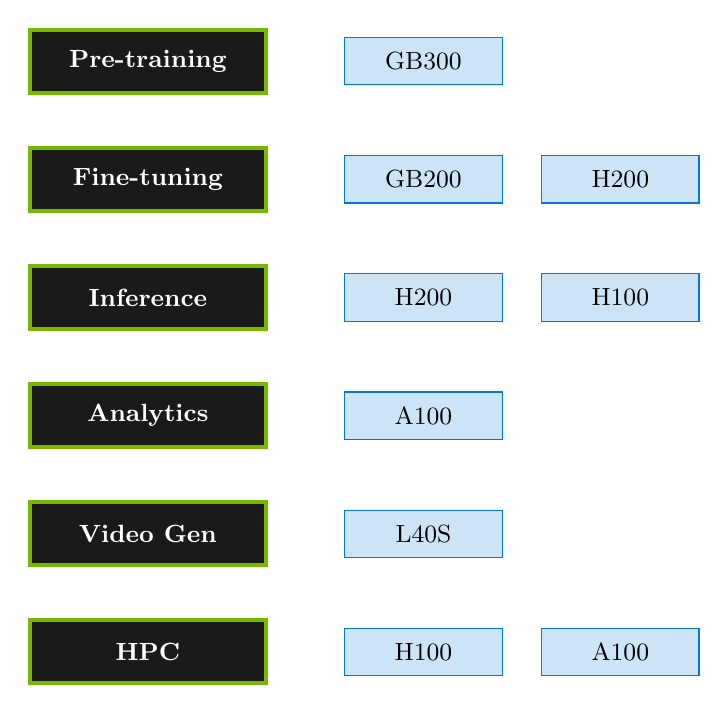
\begin{tikzpicture}[
    node distance=0.5cm,
    workload/.style={rectangle, draw=nvidiagreen, fill=nvidiadarkgray, text=nvidiawhite,
                     minimum width=3cm, minimum height=0.8cm, font=\small\bfseries, line width=1.5pt},
    gpu/.style={rectangle, draw=msblue, fill=msblue!20, text=black,
                minimum width=2cm, minimum height=0.6cm, font=\small}
]
    % Workload categories
    \node[workload] (pretraining) at (0,4) {Pre-training};
    \node[workload] (finetuning) at (0,2.5) {Fine-tuning};
    \node[workload] (inference) at (0,1) {Inference};
    \node[workload] (analytics) at (0,-0.5) {Analytics};
    \node[workload] (video) at (0,-2) {Video Gen};
    \node[workload] (hpc) at (0,-3.5) {HPC};
    
    % GPU recommendations
    \node[gpu, right of=pretraining, xshift=3cm] {GB300};
    \node[gpu, right of=finetuning, xshift=3cm] {GB200};
    \node[gpu, right of=finetuning, xshift=5.5cm] {H200};
    \node[gpu, right of=inference, xshift=3cm] {H200};
    \node[gpu, right of=inference, xshift=5.5cm] {H100};
    \node[gpu, right of=analytics, xshift=3cm] {A100};
    \node[gpu, right of=video, xshift=3cm] {L40S};
    \node[gpu, right of=hpc, xshift=3cm] {H100};
    \node[gpu, right of=hpc, xshift=5.5cm] {A100};
\end{tikzpicture}
\caption{GPU Selection by Workload Type}
\end{figure}

\section{Performance Metrics}

\begin{nvidiabox}[Key Performance Indicators]
\textcolor{nvidiawhite}{
\textbf{When selecting a GPU, consider:}\\[0.3cm]
• \textbf{FP64 Performance:} Scientific computing precision\\
• \textbf{FP32/FP16 Performance:} AI training efficiency\\
• \textbf{INT8 Performance:} Inference throughput\\
• \textbf{Memory Bandwidth:} Data transfer speeds\\
• \textbf{Memory Capacity:} Model size support\\
• \textbf{TDP:} Power consumption requirements
}
\end{nvidiabox}

% ==================== CHAPTER 5: NETWORKING ====================
\chapter{NVIDIA Networking Solutions}

\section{InfiniBand and Ethernet}

High-performance networking is critical for AI infrastructure, enabling efficient multi-GPU and multi-node training.

\begin{table}[H]
\centering
\caption{NVIDIA Networking Technologies}
\begin{tabular}{@{}llll@{}}
\toprule
\textbf{Technology} & \textbf{Bandwidth} & \textbf{Latency} & \textbf{Use Case} \\ \midrule
\textcolor{nvidiagreen}{\textbf{InfiniBand NDR}} & 400 Gb/s & Sub-microsecond & Large-scale training \\
\textcolor{nvidiagreen}{\textbf{Ethernet 400G}} & 400 Gb/s & Low & Cloud deployments \\
\textcolor{msblue}{\textbf{NVLink}} & 900 GB/s & Ultra-low & GPU-to-GPU \\
\textcolor{msblue}{\textbf{NVSwitch}} & 14.4 TB/s & Ultra-low & Multi-GPU systems \\ \bottomrule
\end{tabular}
\end{table}

\section{Multi-GPU Architecture}

\begin{figure}[H]
\centering
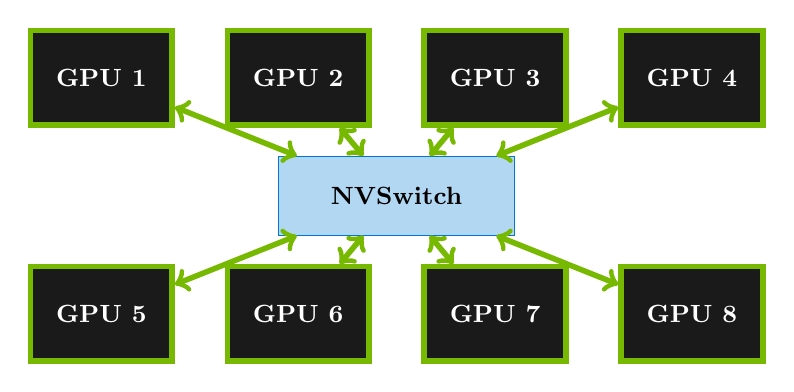
\begin{tikzpicture}[
    gpu/.style={rectangle, draw=nvidiagreen, fill=nvidiadarkgray, text=nvidiawhite,
                minimum width=1.8cm, minimum height=1.2cm, font=\small\bfseries, line width=2pt},
    switch/.style={rectangle, draw=msblue, fill=msblue!30, text=black,
                   minimum width=3cm, minimum height=1cm, font=\small\bfseries}
]
    % GPU Array
    \node[gpu] (gpu1) at (0,3) {GPU 1};
    \node[gpu] (gpu2) at (2.5,3) {GPU 2};
    \node[gpu] (gpu3) at (5,3) {GPU 3};
    \node[gpu] (gpu4) at (7.5,3) {GPU 4};
    
    \node[gpu] (gpu5) at (0,0) {GPU 5};
    \node[gpu] (gpu6) at (2.5,0) {GPU 6};
    \node[gpu] (gpu7) at (5,0) {GPU 7};
    \node[gpu] (gpu8) at (7.5,0) {GPU 8};
    
    % NVSwitch
    \node[switch] (nvswitch) at (3.75,1.5) {NVSwitch};
    
    % Connections
    \foreach \g in {gpu1,gpu2,gpu3,gpu4,gpu5,gpu6,gpu7,gpu8}
        \draw[<->, line width=2pt, color=nvidiagreen] (\g) -- (nvswitch);
\end{tikzpicture}
\caption{NVSwitch Multi-GPU Topology}
\end{figure}

% ==================== CHAPTER 6: SOFTWARE STACK ====================
\chapter{NVIDIA Software Ecosystem}

\section{CUDA Platform}

CUDA (Compute Unified Device Architecture) forms the foundation of NVIDIA's software ecosystem, enabling developers to harness GPU power for parallel computing.

\begin{msbox}[CUDA Capabilities]
\textbf{Key Features:}
\begin{itemize}
    \item Parallel thread execution across thousands of cores
    \item Unified memory architecture
    \item Advanced libraries (cuBLAS, cuDNN, cuFFT)
    \item Multi-GPU and multi-node support
    \item Integration with popular AI frameworks
\end{itemize}
\end{msbox}

\section{AI Framework Support}

\begin{table}[H]
\centering
\caption{NVIDIA-Optimized AI Frameworks}
\begin{tabular}{@{}lll@{}}
\toprule
\textbf{Framework} & \textbf{NVIDIA Optimization} & \textbf{Primary Use} \\ \midrule
\textcolor{nvidiagreen}{\textbf{PyTorch}} & CUDA, cuDNN & Deep Learning \\
\textcolor{nvidiagreen}{\textbf{TensorFlow}} & TensorRT & Production ML \\
\textcolor{msblue}{\textbf{JAX}} & XLA, CUDA & Research \\
\textcolor{msblue}{\textbf{Triton}} & Native GPU kernels & Inference \\
\textcolor{nvidiagreen}{\textbf{RAPIDS}} & cuDF, cuML & Data Science \\ \bottomrule
\end{tabular}
\end{table}

% ==================== CHAPTER 7: CONCLUSION ====================
\chapter{Future Roadmap}

\section{Upcoming Platforms}

\begin{nvidiabox}[Future NVIDIA Platforms]
\textcolor{nvidiawhite}{
\textbf{Rubin Platform (2026):}\\
• Next-generation GPU architecture\\
• Enhanced AI training capabilities\\
• Improved power efficiency\\[0.5cm]

\textbf{Vera Platform (2027+):}\\
• Advanced interconnect technologies\\
• Exascale computing support\\
• Quantum-ready infrastructure
}
\end{nvidiabox}

\section{Industry Impact}

NVIDIA's continuous innovation in GPU technology has fundamentally transformed multiple industries:

\begin{itemize}[label=\textcolor{nvidiagreen}{$\blacktriangleright$}]
    \item \textbf{Artificial Intelligence:} Enabling training of massive language models
    \item \textbf{Scientific Research:} Accelerating drug discovery and climate modeling
    \item \textbf{Autonomous Vehicles:} Powering real-time perception systems
    \item \textbf{Healthcare:} Advancing medical imaging and genomics
    \item \textbf{Financial Services:} High-frequency trading and risk analysis
\end{itemize}

% ==================== REFERENCES PAGE ====================
\chapter*{Resources \& References}
\addcontentsline{toc}{chapter}{Resources \& References}

\section*{Official Documentation}

\begin{itemize}[label=\textcolor{msblue}{$\circ$}]
    \item NVIDIA Data Center GPUs: \url{https://www.nvidia.com/en-us/data-center/}
    \item DGX Systems Documentation: \url{https://docs.nvidia.com/dgx/}
    \item CUDA Toolkit: \url{https://developer.nvidia.com/cuda-toolkit}
    \item NVIDIA Developer Portal: \url{https://developer.nvidia.com/}
\end{itemize}

\section*{GitHub Repositories}

\begin{nvidiabox}[Community Resources]
\textcolor{nvidiawhite}{
\textbf{Explore these repositories for hands-on examples and resources:}\\[0.5cm]

\textbf{1. NvDev Repository}\\
\href{https://github.com/Yash-Kavaiya/NvDev}{\textcolor{nvidiawhite}{https://github.com/Yash-Kavaiya/NvDev}}\\
Comprehensive NVIDIA development resources and examples\\[0.5cm]

\textbf{2. Awesome NVIDIA Repository}\\
\href{https://github.com/Yash-Kavaiya/awesome-nvidia}{\textcolor{nvidiawhite}{https://github.com/Yash-Kavaiya/awesome-nvidia}}\\
Curated list of NVIDIA tools, libraries, and learning resources
}
\end{nvidiabox}

\vspace{1cm}

\begin{center}

\begin{tikzpicture}
    \draw[fill=nvidiadarkgray, draw=nvidiagreen, line width=3pt, rounded corners] 
        (-6,-2) rectangle (6,2);
    \node[text=nvidiawhite, font=\Large\bfseries] at (0,0.8) {Thank You};
    \node[text=nvidiagreen, font=\large] at (0,0) {For Reading This Guide};
    \node[text=nvidialightgray, font=\small] at (0,-0.8) {Created by Yash Kavaiya};
    \node[text=nvidialightgray, font=\small] at (0,-1.2) {Easy AI Labs | Gen AI Guru};
\end{tikzpicture}
\end{center}

\end{document}
